Tools were run on the function \texttt{send\_publish\_notifications(..)} and on the file \texttt{tools.py}.

\paragraph{Pylint}
The Python quality checker \emph{Pylint} is a tool to help with coding standard as recommended by PEP 8, error detection and refactoring.
Pylint message categories:
\begin{itemize}
    \item (C) convention: programming standard violation
    \item (R) refactor: code smell
    \item (W) warning: python specific problem
    \item (E) error: likely bug
    \item (F) fatal: an error occurred preventing pylint from continuing the analysis
\end{itemize}
\begin{figure}[h]
    \centering
    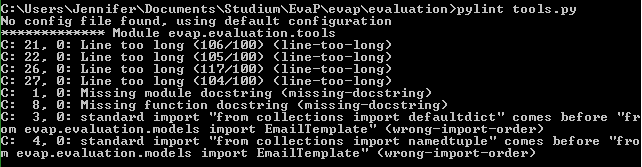
\includegraphics[width=\textwidth, keepaspectratio]{graphics/pylint_send_publish_notifications_1}
    \caption{Pylint messages for \texttt{send\_publish\_notifications(..)}}
    \label{fig:pylint}
\end{figure} 
As expected after our testing Pylint found mostly violated coding conventions in \texttt{send\_publish\_notifications(..)} (\ref{fig:pylint}). 
The investigation of the file \texttt{tools.py} leads to a few warnings and refactoring hints that we will discuss with the developers on the next occasion.
%TODO Restliche Grafiken in den Anhang?


\paragraph{Pychecker}
Even though you still find some outdated recommendations this tool's peak seems to be over. 
The last update was in 2013.
It is written for Python 2.x and has never been ported to Python 3.x.
Since the installation process requires Python 2.x while we work with Python 3.x in EvaP we will drop our investigation with this tool.

\paragraph{pep8}
The Python style guide checker \emph{pep8} checks code against some of the style conventions in PEP 8.
It differentiates between errors and warnings.
\begin{figure}[h]
    \centering
    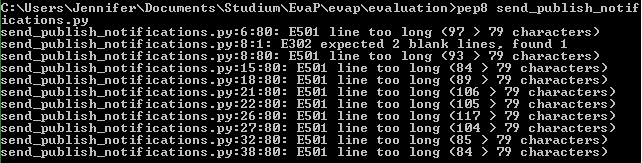
\includegraphics[width=\textwidth, keepaspectratio]{graphics/pep8_send_publish_notifications_1}
    \caption{pep8 messages for \texttt{send\_publish\_notifications(..)}}
    \label{fig:pep8}
\end{figure} 
pep8 throws a few more errors about lines being too long, because the line length was set to 100 instead of 80 characters in Pylint.

\paragraph{Pyflakes}
Unlike Pylint and pep8 \emph{Pyflakes} does not check for violations of coding style but instead focuses on checking for errors.
The tool is less intuitively to use as there is no report if no errors are found. 
It did not report any errors for either \texttt{send\_publish\_notifications(..)} or \texttt{tools.py}

\paragraph{Landscape}
As described above the service Landscape is currently deployed in the development process. 
The service advertises to find errors, possible problems and security issues.
Every time the master branch of the repository is updated Landscape runs several code quality tools including pylint on the whole codebase. 
It accumulates the findings, creates an easy access to them.
A rating based on the findings helps to get an overall idea about the current status.

\begin{figure}[h]
    \centering
    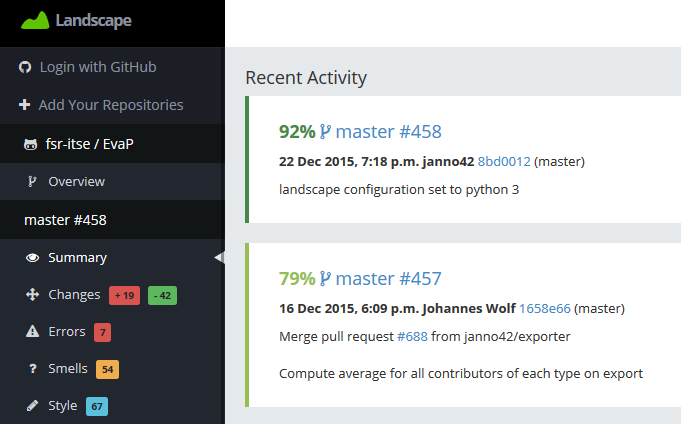
\includegraphics[width=0.7\textwidth, keepaspectratio]{graphics/landscape_python3}
    \caption{Landscape's rating of the code after changing the configuration from Python 2.x to Python 3.x}
    \label{fig:landscape_python3}
\end{figure} 

During our first investigation of the tool, we noticed that something was off about its configuration.
The last run was in %TODO
even though code was pushed to the master branch since then.
Additionally Landscape was still configured to run its checks against Python 2.x while EvaP already made the switch to Python 3.x.
Thankfully a fix of the configuration gave a significant boost to the rating (\ref{fig:landscape_python3}).

\begin{figure}[h]
    \centering
    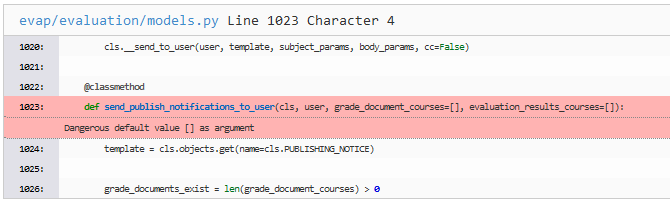
\includegraphics[width=\textwidth, keepaspectratio]{graphics/landscape_error}
    \caption{Landscape's display of an error found with static analysis}
    \label{fig:landscape_error}
\end{figure} 

As we checked out the erros found section, we noticed that one of the found errors actually might have an impact on the function \texttt{send\_publish\_notifications} that we tested earlier. 
Landscape notified that the method \texttt{send\_publish\_notifications\_to\_user} has a dangerous default value as an argument.
This method is called by our function.
%TODO Description why it's dangerous
%TODO Thankfully no failure in the live system
%TODO distinction between fault, error, failure
%TODO Decsription of fix

\paragraph{PyCharm}
%TODO 

\paragraph{Experiences summarized}
Out of the tested tools three were particularly useful.

\begin{itemize}
    \item Pylint is pretty verbose, but very helpful if you are working on adjusting one file to the style guide.
    Its report is especially nice because it delivers statistics about the previous and the current run to compare the improvements due to the last code changes.
    \item PyCharm is especially useful for developers, because its inspection leads to the source code itself.
    Additionally PyCharm suggests fixes for its findings which enhances and accelerates the process quite a lot.
    \item Landscape's advantage is its setup as a service. It allows everyone to get an overview over the code quality without installing a tool on their machine. Furthermore, its automatic run after every code change on the master allows comparison between two states.
\end{itemize}

It is unfortunate that a tool as PyChecker that has not been updated for a while and does not work for Python 3.x is still listed and even highly recommended.  
While the tools pep8 and Pyflakes were not outstandingly useful for us they seem to serve their purpose.

The tools' usefulness regarding testing differs as well:
\begin{enumerate}
    \item PyCharm is the most useful, because it is simultaneously the IDE
    \item Landscape is helpful as it does not only locate possible erros, but suggest why a tester should be rethink the code or write a test 
    \item pylint and pep8 are great, because a uniform code style helps new developers and testers to easily find into the project. 
\end{enumerate}






